\section{Attivit\`a}

Di seguito elenchiamo le attivit\`a individuate in ciascuna fase di sviluppo.
L'interdipendenza fra le attivit\`a di ciascuna fase e il loro progresso sono rappresentati con in forma tabulare, con reti di attivit\`a e con diagrammi di Gantt.

La dipendenza fra le varie attivit\`a non implica la sequenzialit\`a fra queste: per accelerare i tempi di sviluppo del software attivit\`a interdipendenti sono portate avanti contemporaneamente.
In caso di modifiche ai documenti prodotti da una certa attivit\`a vengono svolte ulteriori iterazioni delle altre attivit\`a.
In altre parole all'interno delle singole iterazioni viene adottata una pratica di sviluppo \emph{agile}.

\subsection{Attivit\`a della fase di Inception}

Le attivit\`a individuate come componenti della fase di Inception sono le seguenti:
\begin{description}
	\item[Analisi del contesto]
		Raccolta di informazioni riguardanti il dominio dell'applicazione in sviluppo, in particolare informazioni sui servizi offerti ai privati dagli istituti bancari.
	\item[Studio di fattibilit\`a]
		Determinare in quali condizioni il progetto che si vuole sviluppare \`e realizzabile, in particolare determinare in quali condizioni il software avr\`a mercato e produrr\`a utile per gli sviluppatori.
	\item[Definizione dei requisiti]
		Identificazione dei requisiti utente.
	\item[Specifica dei requisiti]
		Identificazione dei requisiti di sistema.
	\item[Identificazione e specifica business-cases]
		Identificazione dei business-cases del dominio dell'applicazione.
	\item[Identificazione degli use-case principali]
		Identificazione delle famiglie di use-cases presenti nel sistema.
	\item[Individuazione dei rischi]
		Identificazione dei rischi presenti durante il processo software, e contestuale realizzazione di piani di monitoraggio, mitigazione e mantenimento.
	\item[Analisi dei costi]
		Fasi iniziali dell'analisi dei costi: scelta della tecnica di stima e prime misurazioni.
	\item[Stesura dei documenti]
		Produzione di documenti attestanti i progressi fatti nella fase di Inception.
		In particolare:
		\begin{itemize}
			\item Stesura documento di analisi del contesto
			\item Stesura documento dei requisiti
			\item Stesura documento di piano di progetto
		\end{itemize}
\end{description}
Una rappresentazione delle dipendenze fra le attivit\`a \`e fornita dalla tabella in figura \ref{fig:attivita_inception_tabella}, assieme a una misura approssimativa del tempo richiesto da ciascuna attivit\`a.
Il grafo delle dipendenze fra le varie attivit\`a \`e mostrato in figura \ref{fig:attivita_inception_grafo}.

I codici identificativi assegnati e il raggruppamento nel grafo sottolineano la partizione delle attivit\`a in tre sotto-gruppi, uno per documento prodotto.
Gli archi tratteggiati nella rete delle attivit\`a rappresentano dipendenze fra documenti differenti.
Il lavoro ai documenti \`e stato pianificato seguendo queste dipendenze.

\begin{figure*}[!h]
\centering
\begin{tabular}{*{4}{l}}
\toprule
\cellcolor{color2!10} ID & \cellcolor{color2!10} Nome & \cellcolor{color2!10} Durata (sett.) & \cellcolor{color2!10} Dipendenze \\
\midrule
\code{I.AC.1} & Analisi contesto & 3 & --- \\
\code{I.AC.2} & Sviluppo business-cases & 2 & \code{I.AC.1} \\
\code{I.AC.3} & Studio di fattibilit\`a & 4 & \code{I.AC.1} \\
\midrule
\code{I.R.1} & Definizione requisiti & 5 & \code{I.AC.2}  \\
\code{I.R.2} & Specifica requisiti & 3 & \code{I.R.1} \\
\code{I.R.3} & Creazione glossario & 2 & \code{I.R.1}, \code{I.R.2} \\
\code{I.R.4} & Definizione use-case principali & 1 & \code{I.R.1}, \code{I.R.2} \\
\midrule
\code{I.PP.1} & Definizione milestone fasi di progetto & 1 & --- \\
\code{I.PP.2} & Analisi dei rischi & 2 & \code{I.AC.1} \\
\code{I.PP.3} & Analisi dei costi & 2 & \code{I.AC.1}, \code{I.R.2}, \code{I.R.4} \\
\midrule
\code{I.AC} & Stesura documento analisi del contesto & 3 & \code{I.AC.1}, \code{I.AC.2}, \code{I.AC.3} \\
\code{I.R} & Stesura documento dei requisiti & 2 & \code{I.R.1}, \code{I.R.2}, \code{I.R.3}, \code{I.R.4} \\
\code{I.PP} & Stesura documento di piano di progetto & 2 & \code{I.PP.1}, \code{I.PP.2} \\
\bottomrule
\end{tabular}
\caption{\label{fig:attivita_inception_tabella}Rappresentazione tabellare delle attivit\`a della fase di Inception.}
\end{figure*}

\begin{figure*}[!htb]
	\centering
	\caption{Grafo delle dipendenze fra le attivit\`a della fase di Inception.}
	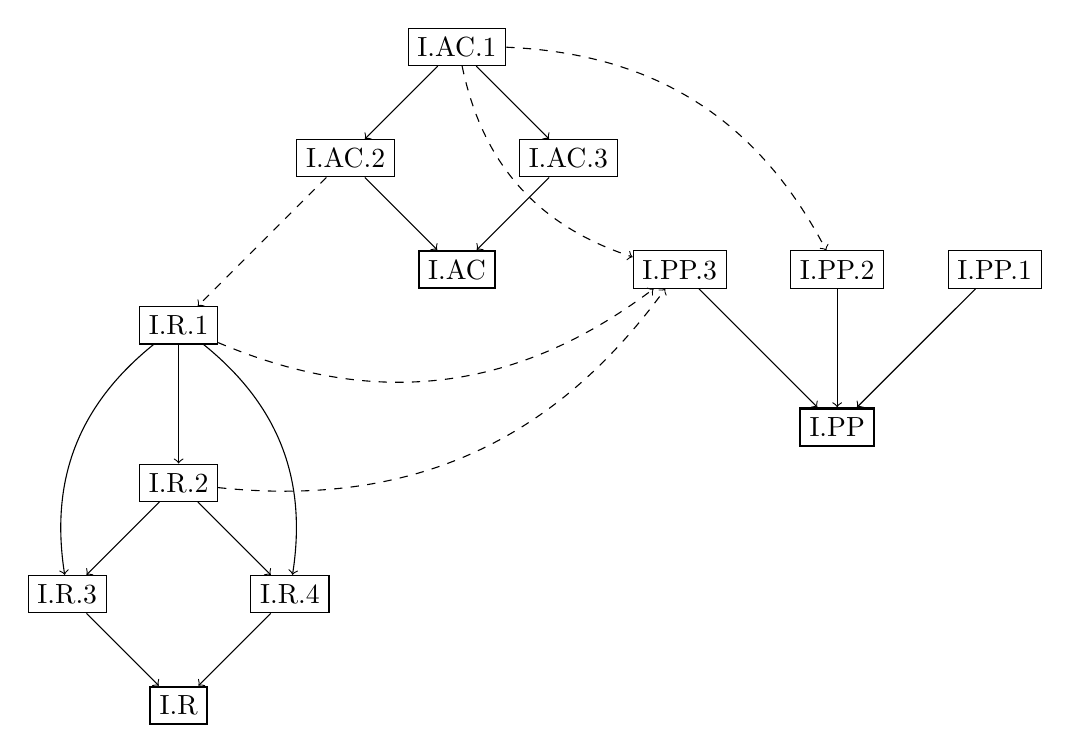
\begin{tikzpicture}[->, node distance=2cm]
		\node[draw=black] (iac1) {\code{I.AC.1}};
		\node[draw=black] (iac2) [below left of=iac1] {\code{I.AC.2}};
		\node[draw=black] (iac3) [below right of=iac1] {\code{I.AC.3}};
		\node[draw=black, thick] (iac) [below right of=iac2] {\code{I.AC}};

		\path (iac1) edge (iac2)
				(iac1) edge (iac3)
				(iac2) edge (iac)
				(iac3) edge (iac);
				
		\node[draw=black] (ir1) [below left of=iac2, node distance=3cm] {\code{I.R.1}};
		\node[draw=black] (ir2) [below of=ir1] {\code{I.R.2}};
		\node[draw=black] (ir3) [below left of=ir2] {\code{I.R.3}};
		\node[draw=black] (ir4) [below right of=ir2] {\code{I.R.4}};
		\node[draw=black, thick] (ir) [below right of=ir3] {\code{I.R}};
		
		\path (iac2) edge [dashed] (ir1);
		
		\path (ir1) edge (ir2)
				(ir1) edge [bend right] (ir3)
				(ir1) edge [bend left] (ir4)
				(ir2) edge (ir3)
				(ir2) edge (ir4)
				(ir3) edge (ir)
				(ir4) edge (ir);

		\node[draw=black] (ipp3) [below right of=iac3] {\code{I.PP.3}};
		\node[draw=black] (ipp2) [right of=ipp3] {\code{I.PP.2}};
		\node[draw=black] (ipp1) [right of=ipp2] {\code{I.PP.1}};
		\node[draw=black, thick] (ipp) [below of=ipp2] {\code{I.PP}};
		
		\path (iac1) edge [dashed, bend left] (ipp2);
		\path (iac1) edge [dashed, bend right] (ipp3)
				(ir1) edge [dashed, bend right] (ipp3)
				(ir2) edge [dashed, bend right] (ipp3);
		
		\path (ipp1) edge (ipp)
				(ipp2) edge (ipp)
				(ipp3) edge (ipp);
	\end{tikzpicture}
	\label{fig:attivita_inception_grafo}
\end{figure*}
